\chapter{A Regularized Cox’s Hierarchical Model for Incorporating Annotation Information in Omics Studies}
\label{cha:xrnetcox}

\section{Abstract}
Associated with high-dimensional omics data there are often “meta-features” such as pathways and functional annotations that can be informative for predicting an outcome of interest. We extend to Cox regression the regularized hierarchical framework of Kawaguchi et al. (2021) for integrating meta-features, with the goal of improving prediction and feature selection performance with time-to-event outcomes. Regularization is applied to the omic features as well as the meta-features so that high-dimensional data can be handled at both levels. The proposed hierarchical Cox model can be efficiently fitted by a combination of iterative reweighted least squares and cyclic coordinate descent. In a simulation study we show that when the external meta-features are informative, the regularized hierarchical model can substantially improve prediction performance over standard regularized Cox regression. Importantly, when the external meta-features are uninformative, the prediction performance based on the regularized hierarchical model is on par with standard regularized Cox regression, indicating robustness of the framework. We illustrate the proposed model with applications to prediction of breast cancer survival, prediction of overall survival of melanoma, based on gene expression.

\section{Introduction}
Prediction based on high-dimensional omics data such as gene expression, methylation, and genotypes are important for developing better prognostic and diagnostic signatures of health outcomes. However, developing prediction models with high-dimensional omics data, where the number of features is often orders of magnitude larger than the available number of subjects is challenging. Sparse regularized regression methods, including the Lasso \citep{tibshirani1996regression} and its variants, elastic net \citep{zou2005regularization}, adaptive Lasso \citep{zou2006adaptive}, group Lasso \citep{yuan2006model} and others, control model complexity by shrinking all regression coefficients toward zero while setting some exactly to zero, effectively selecting features associated with the outcome. 

Kawaguchi et al. (2021) have shown that incorporating meta-features relating to the omics features can yield improved prediction of an outcome of interest and they developed a regularized hierarchical regression framework to incorporate external meta-feature information into the analysis of omics data. Example of meta-features are biological pathways containing different gene sets, functional information from databases like gene ontology, or results and summary statistics from previous studies. Their approach is implemented to handle quantitative and binary outcomes. The regularization type they applied to both features and meta-features is ridge only. Here we extend the regularized hierarchical model of Kawaguchi et al. (2021) to handle time to event outcomes and also add the lasso, elastic net to meta-features.

There are numerous approaches for testing enrichment of meta-features after an analysis relating the genomic features to an outcome of interest is performed. For example, \cite{subramanian2005gene} developed gene set enrichment analysis (GSEA) to yield insights on gene group level. The genes in a group, which is a meta-feature of the genes, share common chromosomal location or biological function. The enrichment analysis is performed after prior analysis of single gene differential expression analysis. However, there are few approaches capable of incorporating meta-features directly into the modeling process, rather than in a post-hoc fashion. Approaches to incorporate meta-features include the application of differential penalization based on external information and two-stage regression methods, where the outcome is first regressed on the genomic features and the resulting effect estimates are in turn regressed on the external meta features. \cite{tai2007incorporating} grouped genes based on existing biological knowledge and applied group-specific penalties to nearest shrunken centroids and penalized partial least squares. \cite{bergersen2011weighted} incorporates external meta-feature information by weighting the LASSO penalty of each genomic feature with some function of meta-feature. \cite{zeng2021incorporating} on the other hand, incorporates external meta-feature to customize the penalty of each feature with a different function of meta-feature. These three methods are based on idea 1), which no longer assuming every genomic feature are equally important, but of different importance based on external information. However, they cannot handle large number of meta-features. \cite{chen2007enriching} applied the idea of hierarchical modeling in a Bayesian framework, where second stage linear regression is normal prior distribution, first stage regression is normal conditional distribution, and estimate first stage regression coefficients with posterior estimator. This method does not apply to high dimensional data since it is standard regression with no regularization. The above data integration methods improve prediction compared to modeling with genomic features only. However, none of the approaches above can handle time-to-event outcomes.

In this chapter, we introduce a regularized Cox’s proportional hazard hierarchical model to integrate meta-features. We will see that when external meta-features are informative, regularized hierarchical modeling improves prediction performance considerably. On the other hand, we also show that when the external meta-features are not informative, it does not perform worse than standard regularized model, which does not use any external information. This shows that the model is robust to the informativeness of the meta-features and can be safely used when the meta-feature informativeness is a priori unknown, as it is typically the case. The model can be efficiently fitted using a combination of iterative reweighted least squares and cyclic coordinate descent as proposed for Lasso Cox regression by \cite{simon2011regularization}.

\section{Methods}
\subsection{Setup and notation}
We assume a survival analysis setting with outcome $(\bm{y},\bm{\delta})=(y_1,\dots,y_n,\delta_1,\dots,\delta_n)$, where $\bm{\delta}=(\delta_1,\dots,\delta_n)$ is a vector of censoring status for each subject, $\delta_i=1$ represents event happens, $\delta_i=0$ represents right-censoring; $\bm{y}=(y_1,\dots,y_n)$ is the vector of observed time, if $\delta_i=1$, $y_i$ is event time, and if $\delta_i=0$, $y_i$ is censoring time, for $n$ subjects. Let $\bm{X}$ denote the $n\times p$ design matrix, where $p$ is the number of features, each row represents the observations on one subject, and each column represents the values of one feature across the $n$ subjects. We are particularly interested in the high dimension setting, $p>>n$, where the number of features is larger than the sample size. The goal is to develop a predictive model for the outcome $(\bm{y},\bm{\delta})$ based on the data $\bm{X}$.

In a genomics context, the time-to-event outcome $(\bm{y},\bm{\delta})$ could be event free time, time to disease relapse, time to death. The design matrix $\bm{X}$ could be genotypes, gene expressions, DNA methylation. For example, in Molecular Taxonomy of Breast Cancer International Consortium (METABRIC) data, outcome $(\bm{y},\bm{\delta})$ is breast cancer specific survival, data matrix $\bm{X}$ represents gene expressions with dimension number of patients$\times$number of genes.

Associated with each feature there is typically a set of meta-features annotations. If $\bm{X}$ consists of gene expression values, pathway gene sets could be meta-features indicating the set of genes involved. As for the METABRIC example, 4 meta-features are believed to be associated with breast cancer: genes with mitotic chromosomal instability (CIN), mesenchymal transition (MES), lymphocyte-specific immune recruitment (LYM), and FGD3-SUSD3 genes. Each meta-feature consists a vector of indicator variables for whether a gene belongs to the functional gene group. The genomic meta-features can be collected into a matrix $\bm{Z}$ of dimensions $p\times q$, where $q$ is the number of meta-features. We propose a penalized hierarchical regression for integrating the external meta-feature information in $\bm{Z}$ for predicting time-to-event outcomes based on the features in $\bm{X}$
\begin{equation}
    \min_{\bm{\alpha},\bm{\beta}} \left\{ -\frac{1}{n}\ln{L_B(\bm{\beta})}+\frac{\lambda_1}{2}\|\bm{\beta}-\bm{Z\alpha}\|_2^2+\lambda_2\|\bm{\alpha}\|_1 \right\}, \label{eq2.1}
\end{equation}
where $L_B(\bm{\beta})$ is the negative log of the Cox partial likelihood function (see below), $\bm{\beta}$ is a length $p$ vector of regression coefficients corresponding to the $p$ features in $\bm{X}$, and $\bm{\alpha}$ is a length $q$ vector of regression coefficients corresponding to the meta-features. The objective function in \eqref{eq2.1} can be viewed as arising from a hierarchical model. In the first level of the hierarchy, the negative log partial likelihood $L_B(\bm{\beta})$ term in \eqref{eq2.1} corresponds to the time-to-event outcome modeled as a function of $\bm{X}$ via a Cox’s proportional hazard regression model. In the second level, the $L_2$ penalty term $\|\bm{\beta}-\bm{Z\alpha}\|_2^2$ corresponds to a linear regression of the estimate of $\bm{\beta}$ on the meta-feature information $\bm{Z}$. It can also be thought of as an $L_2$ regularization term that shrinks the estimate of $\bm{\beta}$ toward $\bm{Z\alpha}$ rather than to the usual shrinkage toward zero. In the third level of the hierarchy, the term $\|\bm{\alpha}\|_1$ is an $L_1$ regularization penalty on the vector of estimated efficts $\hat{\bm{\alpha}}$. It enables the selection of important meta-features by shrinking many of its components to $0$. The hyperparameters $\lambda_1,\lambda_2\geq0$ control the degree of shrinkage/regularization applied to each of the penalty terms and can be tuned by cross-validation. Finally, note that when $\bm{\alpha}=0$, the objective function \eqref{eq2.1} reduces to a standard $L_2$-regularized Cox regression.

The partial likelihood function $L_B(\bm{\beta})$ in \eqref{eq2.1} is the Breslow approximation \citep{breslow1972contribution} to the Cox partial likelihood. Letting $t_1<t_2<\cdots<t_k (k=1,2,\dots,D)$ be unique event times arranged on increasing order, the Cox model assumes proportional hazards: 
\begin{equation}
    h(t,\bm{x}_j)=h_0(t)\exp{(\bm{x}_j^T\bm{\beta})}, \label{eq2.2} 
\end{equation}
where $h(t,\bm{x}_j)$ is the hazard rate for subject $j$ with feature values $\bm{x}_j$ at time $t$; $h_0(t)$ is baseline hazard rate at time $t$, regardless of the feature values. The Cox partial likelihood function \citep{cox1972regression} can then be written as
\begin{equation}
    L(\bm{\beta})=\prod_k \frac{e^{\bm{x}_k^T\bm{\beta}}}{\sum_{j\in R_k}e^{\bm{x}_j^T\bm{\beta}}}, \label{eq2.3}
\end{equation}
where $R_k=\{j:y_j\geq t_k\}$, is the risk set at time $t_k$, i.e., the set of all subjects who have not experienced the event and are uncensored just prior to time $t_k$. The partial likelihood function allows estimation of $\bm{\beta}$ without explicitly modeling the baseline $h_0$, and it depends only on the order in which events occur but not on the exact times of occurrence. However, the partial likelihood assumes that event times are unique. To handle ties, where multiple individuals experience the event at the same time, we use the Breslow approximation of the partial likelihood in \eqref{eq2.3}
\begin{equation}
    L_B(\bm{\beta})=\prod_k \frac{\exp{(\sum_{j\in D_k}\bm{x}_k^T\bm{\beta})}}{(\sum_{j\in R_k}e^{\bm{x}_k^T\bm{\beta}})^{d_k}}, \label{eq2.4}
\end{equation}
where $D_k=\{j:\delta_j=1,y_j=t_k\}$, is the set of individuals who have event time $y_k$, and $d_k=\sum_jI(\delta_j=1,y_j=t_k)$ is the number of events at time $y_k$. Breslow’s likelihood function automatically reduces to the partial likelihood when there are no ties. 

\subsection{Model fitting}
The objective function \eqref{eq2.1} can be minimized efficiently using iterative reweighted least squares combined with coordinate descent \citep{simon2011regularization}. If the current estimates of the regression coefficients are $(\tilde{\bm{\beta}}, \tilde{\bm{\alpha}})$, we form a quadratic approximation to the negative log-partial likelihood by Taylor series around the current estimates. The approximated objective function has the form:
\begin{equation}
    \min_{\bm{\alpha},\bm{\beta}} \left\{ -\frac{1}{2n}(\bm{y}'-\bm{X\beta})^T\bm{W}(\bm{y}'-\bm{X\beta})+\frac{\lambda_1}{2}\|\bm{\beta}-\bm{Z\alpha}\|_2^2+\lambda_2\|\bm{\alpha}\|_1 \right\}, \label{eq2.5}
\end{equation}
where 
\begin{equation}
    \bm{y}'=\tilde{\bm{\eta}}+\bm{W}^{-1}(\bm{\delta}-\text{diag}[\exp{(\ln{H_0(\bm{y})}+\tilde{\bm{\eta}})}]), \label{eq2.6} 
\end{equation}
\begin{equation}
    \bm{W}=\text{diag}\left[\exp{(\ln{H_0(\bm{y})}+\tilde{\bm{\eta}})}\right] - \text{diag} [e^{\tilde{\bm{\eta}}}]\bm{M}\text{diag}\left[\frac{h_{0k}^2}{d_k}\right]\bm{M}^T\text{diag}[e^{\tilde{\bm{\eta}}}]. \label{eq2.7}
\end{equation}
In \eqref{eq2.6} and \eqref{eq2.7}, $\text{diag}[\bm{a}]$ is a diagonal matrix with vector $\bm{a}$ as diagonal elements. $\bm{M}$ is an $n\times D$ indicator matrix with $(i,k)^{th}$ element $I(y_i\geq t_k)$. Also, $\tilde{\bm{\eta}}=\bm{X}\tilde{\bm{\beta}}$ is the linear predictor; $h_{0k}=\frac{d_k}{\sum_{j\in R_k}\exp{(\tilde{\eta}_j)}}$ is estimated baseline hazard rate at event time $y_k$; $H_0(y_i)=\sum_{k:y_k\leq y_i}h_{0k}$ is cumulative baseline hazard at time $y_i$. In the first part of quadratic approximation \eqref{eq2.5}, $-\frac{1}{2n}(\bm{y}'-\bm{X\beta})^T\bm{W}(\bm{y}'-\bm{X\beta})$ can be viewed as a weighted version of least squares as $\bm{y}'$ work as responses, $\bm{W}$ as weights. Weight matrix $\bm{W}$ is usually a diagonal matrix, however, in Cox proportional hazard model, $\bm{W}$ is a full symmetric matrix as shown in \eqref{eq2.7}. This leads to computational difficulty as it requires calculation of $O(n^2)$ entries. According to \cite{simon2011regularization}, we can compute only the diagonal entries of $\bm{W}$ without much loss of accuracy, thereby speeding up implementation. The diagonal elements of $\bm{W}$, $w_i$ has the form:
\begin{equation}
    w_i=\sum_{k\in C_i}\frac{d_k e^{\tilde{\eta}_i}}{\sum_{j\in R_i}e^{\tilde{\eta}_j}}-\sum_{k\in C_i}\frac{d_k (e^{\tilde{\eta}_i})^2}{(\sum_{j\in R_i}e^{\tilde{\eta}_j})^2}, \label{eq2.8}
\end{equation}
where $C_i$ is the set of unique event time $t_k$ such that $t_k<y_i$ (the times for which observation $i$ is still at risk). In computing weights $w_i$’s, one bottleneck is that for each $k$ in $C_i$, we need to calculate $\sum_{j\in R_i}e^{\tilde{\eta}_j}$. Both $C_i$ and $R_k$ have $O(n)$ elements, so the weight computation is $O(n^2 )$ time. However, if we sort $y_i$’s in non-decreasing order, note that $\sum_{j\in R_i}e^{\tilde{\eta}_j}$ can be calculated in a cumulative summation fashion: for the risk set $R_{k+1}$, the only difference between it and $R_k$ are the observations that are in $R_k$ but not in $R_{k+1}$, ${j: t_k\leq y_j<t_{k+1}}$. This same idea can also be applied to calculate $\sum_{k\in C_{i+1}}\frac{d_k}{\sum_{j\in R_i}e^{\tilde{\eta}_j}}$. And the weight computation complexity can be reduced to $O(n)$. Details are in Appendix \ref{a.1}.

Now, let $\bm{\gamma}=\bm{\beta}-\bm{Z\alpha}$, and use only diagonal elements of $\bm{W}$, then \eqref{eq2.5} can be written as:
\begin{equation}
    \min_{\bm{\alpha},\bm{\beta}} \left\{ \frac{1}{2n} \sum_{i=1}^n w_i(y_i'-\bm{\gamma}^T\bm{x}_i-\bm{\alpha}^T(\bm{XZ})_i)^2+\frac{\lambda_1}{2}\|\bm{\gamma}\|_2^2+\lambda_2\|\bm{\alpha}\|_1 \right\}, \label{eq2.9}
\end{equation}
where $(\bm{XZ})_i$ is the $i^{th}$ row of $n\times q$ matrix $\bm{XZ}$. This reduced the problem to repeatedly solving the regularized, weighted least squares problem \eqref{eq2.9} using cyclic coordinate descent \citep{friedman2010regularization}. Details are given in Appendix \ref{a.2}.

\subsection{Two-dimensional hyperparameter tuning}
The optimization approach described above is for fitting the model for one combination of the tuning parameters $\lambda_1,\lambda_2$. More than one value combination of $\lambda_1,\lambda_2$ are usually of interest, as $\lambda_1,\lambda_2$ are tuned by cross-validation to get the best performance out of the model. For the proposed model, a two-dimensional grid of $\lambda_1,\lambda_2$ values are constructed, and pathwise coordinate optimization \citep{friedman2007pathwise} is applied along the two-dimensional path. The pathwise algorithm utilizes current estimates as warm start, since the solutions to the convex problem \eqref{eq2.9} is continuous. This character makes the algorithm remarkably efficient and stable.

In detail, for $\lambda_1$ of the the two-dimensional grid, which controls the amount of shrinkage to $L_2$ term $\|\bm{\beta}-\bm{Z\alpha}\|_2^2$, or in the transformation form $\|\bm{\gamma}\|_2^2$, since we initialize $\tilde{\bm{\gamma}}=0, \tilde{\bm{\alpha}}=0$, starting with $\lambda_{1\max}=1000\times \max_j\frac{1}{n}\sum_{i=1}^nw_i(0)x_{ij}y'_i(0)$ gives small value solutions to $\hat{\bm{\gamma}},\tilde{\bm{\alpha}}$, making the algorithm faster to converge. While for $\lambda_2$, which controls the amount of shrinkage to $L_1$ term $\|\bm{\alpha}\|_1$, $\lambda_{2\max}=\max_k \frac{1}{n}\sum_{i=1}^n w_i(0)(xz)_{ik}y'_i(0)$ is the smallest value that makes the entire vector $\hat{\bm{\alpha}}=0$. We compute the solutions for a decreasing sequence of $\lambda_1,\lambda_2$. More specifically, we start with $\lambda_{1\max},\lambda_{2\max}$, select $\lambda_{\min}=0.001\lambda_{\max}$, and construct a sequence of 20 $\lambda$ values from $
\lambda_{\max}$ to $\lambda_{\min}$ on log scale, therefore there are 400 $\lambda_1,\lambda_2$ combination of values in total. In order to apply warm start, we fix one value of $\lambda_1^{(m_1)}, 1\leq m_1\leq 20$, decrease $\lambda_2$ along the sequence, but keeping the solutions for $\lambda_{1}^{(m_1)}, \lambda_{2\max}$, so that when we work out the solutions for one sequence of $\lambda_2$ values and go to $\lambda_{1}^{(m_1+1)}, \lambda_{2\max}$, (where $\lambda_{1}^{(m_1+1)}$ is the next value along the sequence of $\lambda_1$), we can use the solutions of $\lambda_{1}^{(m_1)}, \lambda_{2\max}$ for warm start (figure \ref{fig:2d}).
\begin{figure}[tbh]
  \centering
  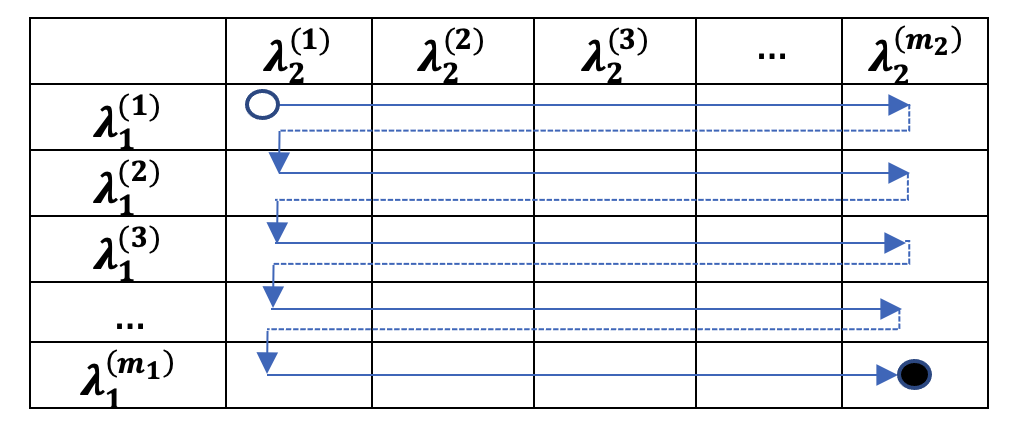
\includegraphics[scale=0.8]{2D-grid}
  \caption[Two-dimensional grid pathwise optimization]{
    Two-dimensional grid pathwise optimization.
  }
  \label{fig:2d}
\end{figure}

\subsection{Summary}
Summarizing procedures for fitting regularized hierarchical Cox model: 
\begin{enumerate}
    \item Initialize $\bm{\beta}$ and $\bm{\alpha}$ with $\widetilde{\bm{\beta}}$ and $\widetilde{\bm{\alpha}}$.
    \item For each $\lambda_1, \lambda_2$, repeat, until convergence of $(\hat{\bm{\beta}},\hat{\bm{\alpha}})$: 
    \begin{itemize}
        \item Compute weights $\bm{W}$ and working response $\bm{y}'$ with current estimate $(\tilde{\bm{\beta}},\tilde{\bm{\alpha}})$, form the quadratic approximation, equation \eqref{eq2.5}
        \item Find minimizer $(\hat{\bm{\beta}},\hat{\bm{\alpha}})$, solution to equation \eqref{eq2.9}, using coordinate descent
        \item Set $(\tilde{\bm{\beta}},\tilde{\bm{\alpha}})=(\hat{\bm{\beta}},\hat{\bm{\alpha}})$
    \end{itemize}
\end{enumerate}

\section{Simulations}
\subsection{Simulation methods}
We performed a simulation study to evaluate the predictive performance of the hierarchical Cox’s regression model compared to standard penalized Cox’s regression. The main parameters we control include informativeness of the meta-features, sample size, number of features and number of meta-features. We generated the $p\times q$ meta-feature matrix $\bm{Z}$, with each element drawn from an independent Bernoulli variable with probability $0.1$. This mimics binary indicators for whether a gene belongs to a particular biological pathway.  

The first level regression coefficients are generated as $\bm{\beta}=\bm{Z\alpha}+\bm{\varepsilon}$, where $\bm{\varepsilon} \sim N(0, \sigma^2\bm{I})$. To control the predictive power of the meta-features, we set the signal-to-noise ratio, $\text{SNR}=\bm{\alpha}^T\text{cov}(\bm{Z})\bm{\alpha}/\sigma^2$, where the signal is the variance of $\bm{\beta}$ explained by model $\bm{Z\alpha}$, and $\sigma^2$ is the noise. A higher signal-to-noise ratio implies a higher level of informativeness of the meta-features with respect to the coefficients $\bm{\beta}$. The data matrix $\bm{X}$ is generated by sampling from a multivariate normal distribution, $N(0,\Sigma)$, where the covariance matrix $\Sigma$ has an autoregressive correlation structure $\Sigma_{ij}=\rho^{|i-j|}$ for $i,j=1,\dots,p$.

The cumulative distribution function of the Cox proportional hazard model is given by
\begin{equation*}
    F(t|\bm{x})=1-\exp\left[-H_0(t)e^{\bm{\beta}^T\bm{x}}\right],
\end{equation*}
where $H_0(t)$ is baseline cumulative hazard function. Using the inverse probability integral transform \citep{bender2005generating}, we generated survival times $t$ as:
\begin{equation}
    t=H_0^{-1}\left[-\ln(U)e^{-\bm{\beta}^T\bm{x}}\right], \label{eq2.10}
\end{equation}
where $U\sim \text{uniform}[0,1]$. For the baseline hazards we used a Weibull distribution, which has cumulative hazard function $H_0(t)=(\frac{t}{b})^v$. The baseline Weibull parameters were set to $b=5,v=8$, which result in survival times in the range $0$ to $20$. We simulated the censoring time, $c$, based on an exponential distribution with density $f(c)=\exp(\lambda c)$, with $\lambda=0.06$. Then, the time-to-event outcome $(y_i,\delta_i)$ is generated as $(\min(t_i,c_i),I(t_i<c_i))$. The value of exponential distribution parameter $\lambda$ was chosen to result in a ratio of subjects experiencing the event vs. subjects experiencing censoring of about $2$ to $1$.

To control the predictivity of the features $\bm{X}$ for the outcome $\bm{y}$, we set Harrell’s concordance index (C-index) \citep{harrell1982evaluating} as the performance metric. It is defined as the probability that a randomly selected patient who experienced an event has a higher risk score $\bm{\beta}^T\bm{x}$ than a patient who has not experienced an event at a given time. The C-index is an analog of the area under the ROC for time-to-event data. The higher the C-index, the better the model can discriminate between subjects who experience the outcome of interest and subjects who do not or have not yet. To control the C-index we added random noise to the survival times $t$, where the noise is distributed as a normal with mean zero and a variance value set to yield a C-index of 0.8 across all simulation scenarios. This is the population/theoretical C-index of the generated survival data, achievable if $\bm{\beta}$ were known or if one had an infinite sample size. When $\bm{\beta}$ is estimated from a finite training set, the achieved model C-index will be lower.

We simulated a base case scenario with sample size $N=100$, number of features $p=200$, and number of meta-features $q=50$. This is a high dimensional setting, $p>>N$, typical of genomic studies. The first 20\% of the coordinates of the meta-feature level coefficients $\bm{\alpha}$ were set to be 0.2, and the rest set to 0. In the base scenario, the meta-features are highly informative, with a signal noise ratio set to 2. The covariance matrix $\bm{\Sigma}$ of $\bm{X}$ has autoregressive-1 structure, parameter $\rho=0.5$, so that the features are moderately correlated. In the following simulation situations, we vary one of the parameters and hold the others fixed. Simulations were performed with $B=100$ replicates for all scenarios. The models were trained on a training set of size $N$ (100 in the base scenario but varied in the experiments below), with the hyper-parameters $\lambda_1,\lambda_2$ tuned on an independent validation set of the same size as training set. The final predictive performance was evaluated on a large test set of size 10,000.

We run a series of experiment varying one key parameter at a time from the base case scenario as follows:

Experiment 1: varying the signal-to-noise ratio of the meta-features from completely uninformative, (SNR$=0$), to slightly informative (SNR$=0.1$), to moderately informative, (SNR$=0.8$), to highly informative (SNR$=2$).

Experiment 2: Varying the sample size from low to high, $N=100,200,500$.

Experiment 3: Varying the number of features from low to high: $p=200,500,1000$.

Experiment 4: Varying the number of meta-features from low to high: $q=20,50,100$.

\subsection{Simulation results}
The results of the experiments are shown in Figure \ref{fig:sim1}. In each panel, the horizontal dashed line representing the population/theoretical C-index, the maximum achievable with infinite training data, is provided as a reference for each parameter setting. We compared the performance of the hierarchical ridge-lasso Cox model incorporating meta-features to that of a standard ridge Cox model.

With informative meta-features (SNR$>0$ in experiments 1-4) the hierarchical ridge-lasso model consistently outperforms the standard ridge model, with the performance gain over the standard ridge model increasing with the informativeness of the meta-features (experiment 1). Importantly, when the meta-features are completely uninformative, the hierarchical ridge-lasso model performs only slightly worse than standard ridge model (experiment 1, SNR$=0$). This shows robustness of the hierarchical ridge-lasso to uninformative meta-features.

Experiment 2 shows that the gains in performance of the hierarchical ridge-lasso over the standard ridge model can be quite large, particularly when the sample size is small. As the sample size $N$ increases, the performance of both models increases and the difference between the two is reduced. 

As the dimensionality $p$ of the features increases (experiment 3), the performance of the standard ridge model deteriorates dramatically, while the performance of the hierarchical model only decreases slowly as the information in the meta-features helps stabilize its performance.

In experiment 4, the performance of the standard ridge model does not change, as it does not utilize meta-feature information. However, for the hierarchical ridge-lasso model, the performance decreases as the number of noise meta-features increases (the number of informative meta-feature is fixed at 10 and the additional meta-features are noise meta-features).  
\begin{figure}[tbh]
  \centering
  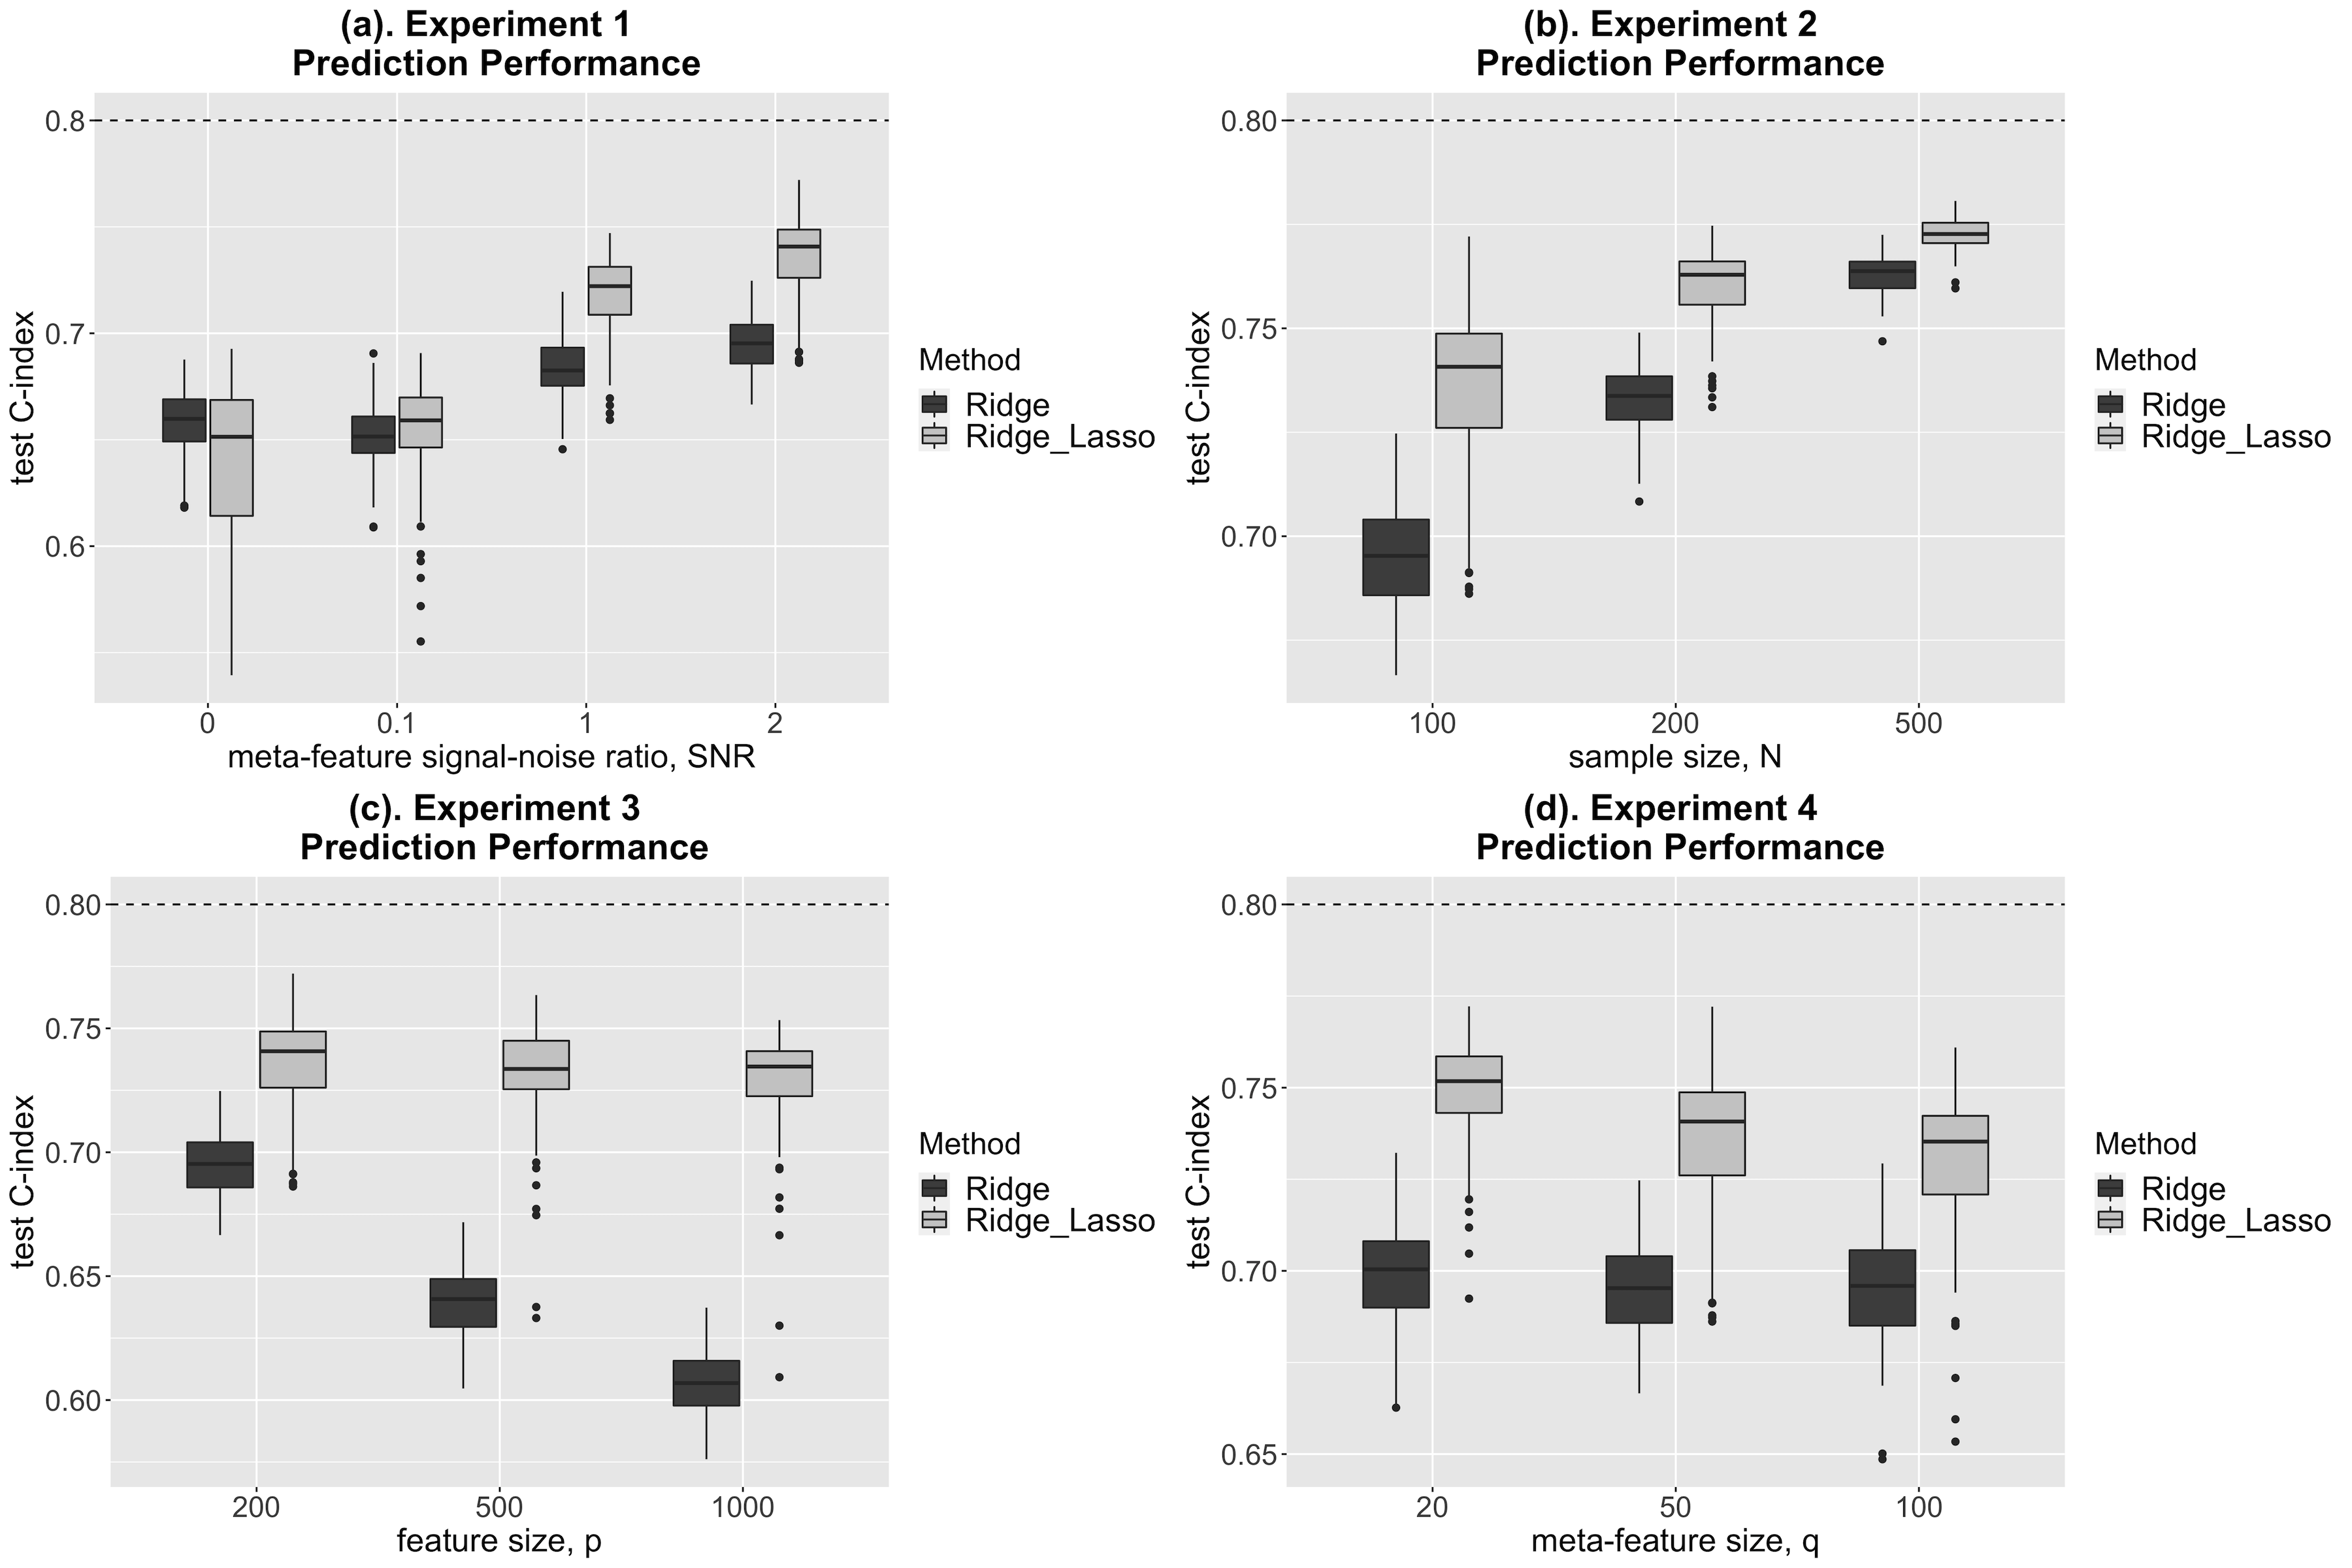
\includegraphics[width=\textwidth]{sim1}
  \caption[Simulation results (`xrnet'): prediction performance]{
    Simulation results: prediction performance.
  }
  \label{fig:sim1}
\end{figure}

We also examined the ability of the model to select informative meta-features by second-level Lasso penalty. In particular, we looked at the true and false positive meta-feature selection rate in experiment 1, where the second level meta-features informativeness varies (Figure \ref{fig:sim2}). We see that as the SNR of the meta-features increases, the true positive selection rate of informative meta-features improves dramatically (Figure 2.3a) at the cost of a slight increase in the false positive rate (Figure 2.3b).  
\begin{figure}[tbh]
  \centering
  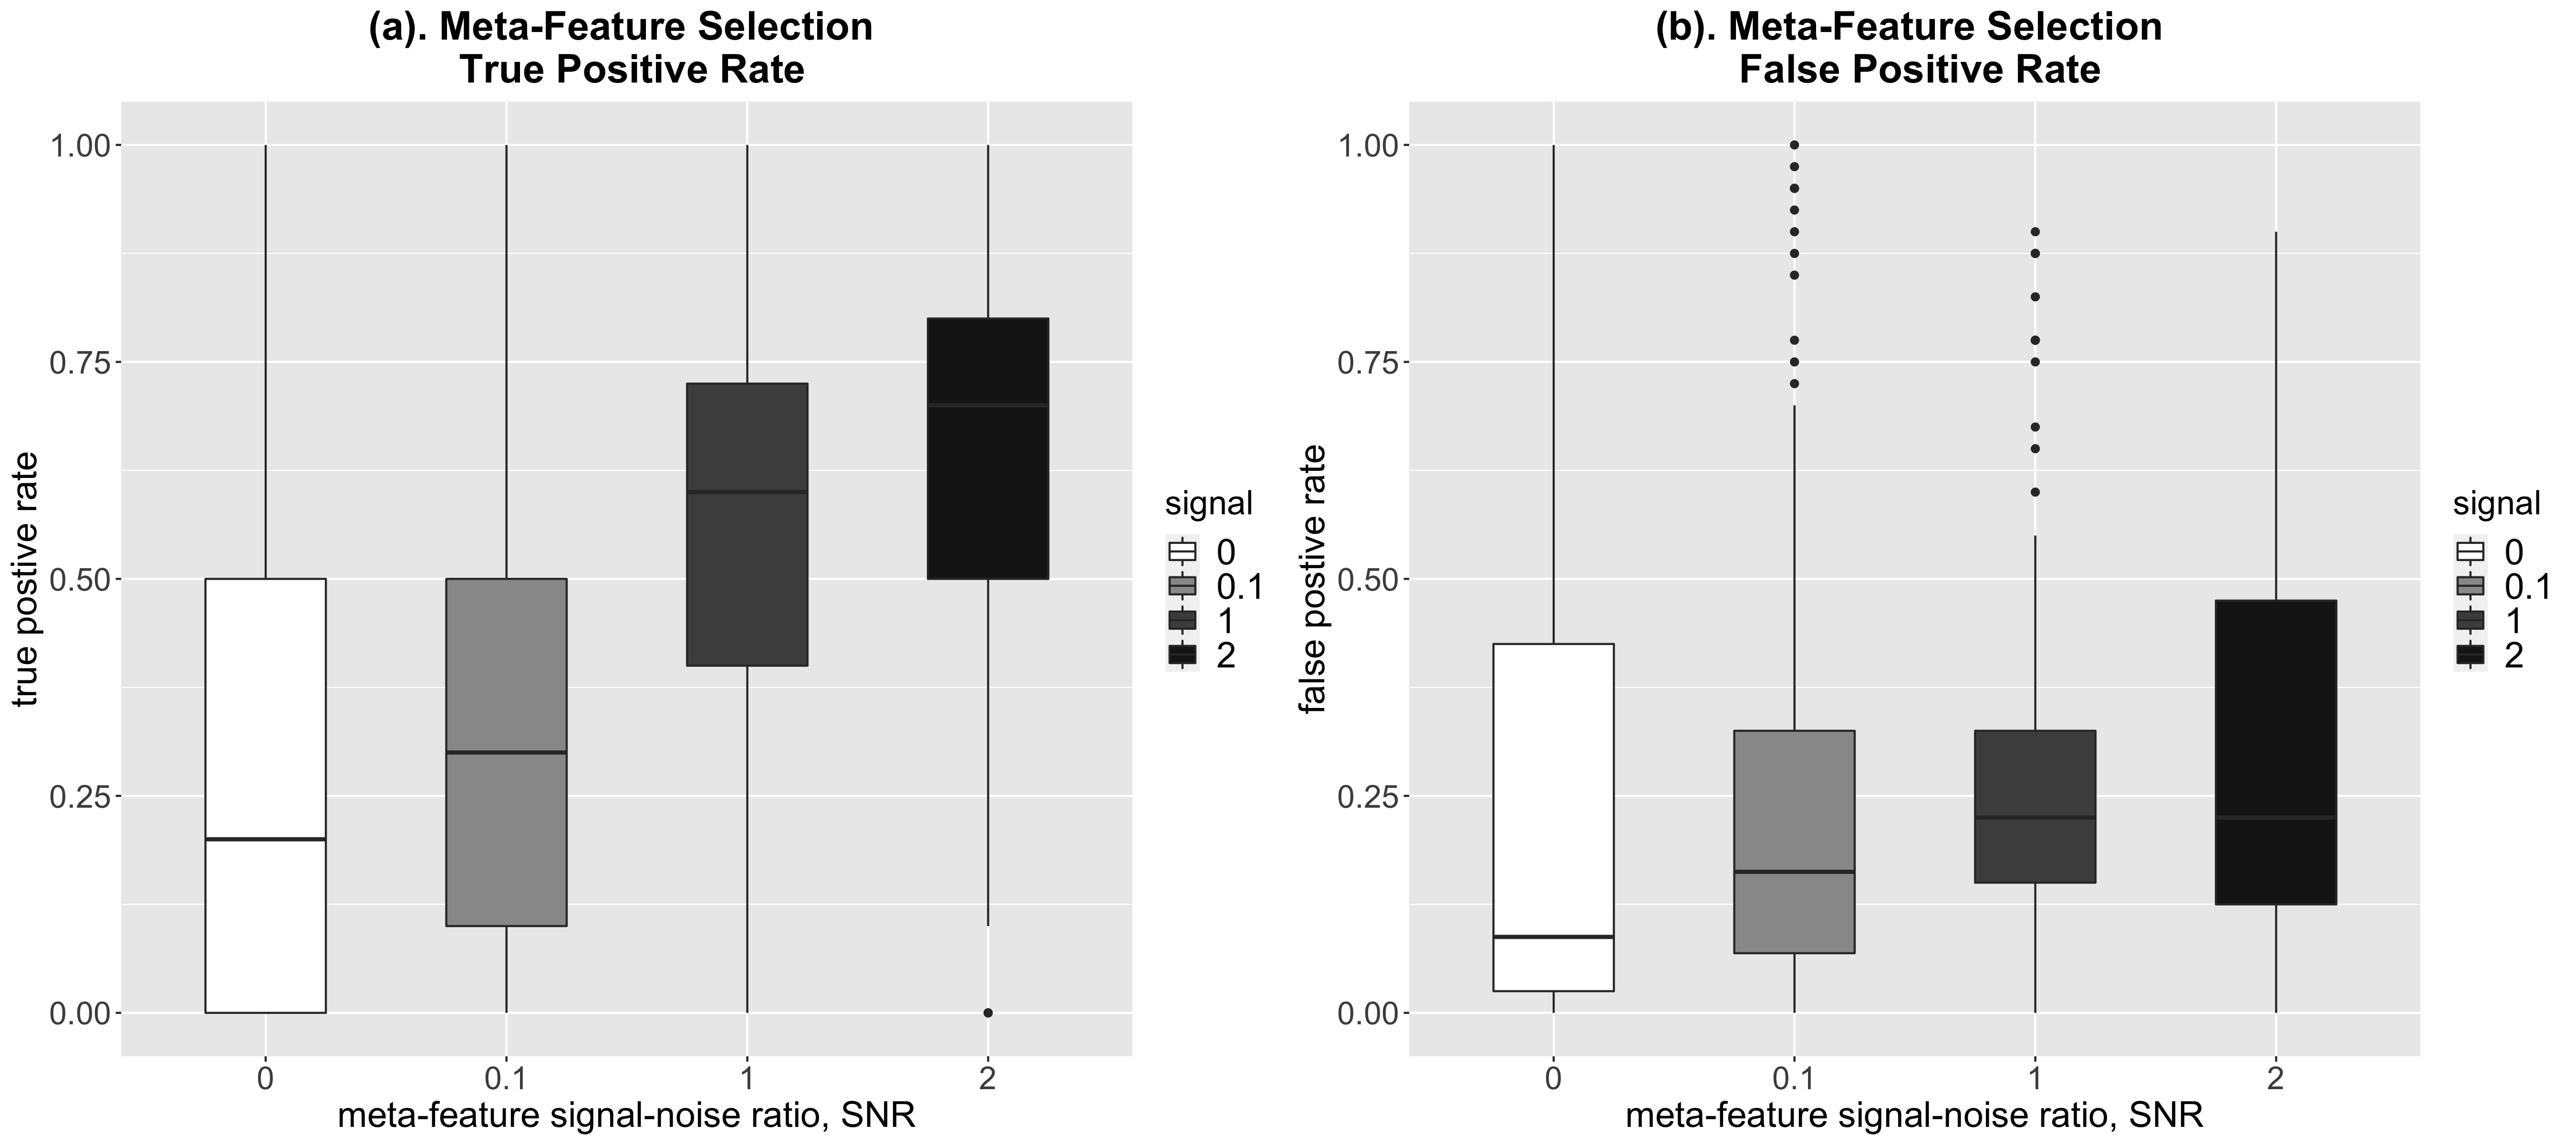
\includegraphics[width=\textwidth]{sim2}
  \caption[Simulation results (`xrnet'): meta-feature selection]{
    Simulation results: meta-feature selection.
  }
  \label{fig:sim2}
\end{figure}

\section{Applications} \label{app:meta2}
\subsection{Gene expression signatures for breast cancer survival}
To illustrate the performance of our approach, we applied the hierarchical survival model to the Molecular Taxonomy of Breast Cancer International Consortium (METABRIC) study. The METABRIC microarray dataset is available at European Genome-Phenome Archive with the accession of EGAS00000000083. It includes cDNA microarray profiling of around 2000 breast cancer specimens processed on the Illumina HT-12 v3 platform (Illumina\_Human\_WG-v3) \citep{curtis2012genomic}. The dataset was divided into a discovery/training set of 997 samples, and a validation/test set of 995 samples \citep{cheng2013development}. The goal is to build a prognostic model for breast cancer survival, based on gene expressions and clinical features. The data $\bm{X}$ consists of of 29,477 gene expression probes and two clinical features, age at diagnosis and the number of positive lymph nodes. The meta-feature data $\bm{Z}$ consists of four ``attractor metagenes'', which are selected gene co-expression signatures that are associated with the ability of cancer cells to divide uncontrollably, to invade surrounding tissues, and, with the effort of the organism to fight cancer with a particular immune response \citep{cheng2013biomolecular}. The three universal “attractor metagenes” are genes involved in mitotic chromosomal instability (CIN), in mesenchymal transition (MES), lymphocyte-specific immune recruitment (LYM). In addition, a meta-gene whose expression is associated with good prognosis and that contains the expression values of two genes—FGD3 and SUSD3. The CIN, MES, and LYM metagenes each consist of 100 genes, but for our analysis, we only considered the 50 top-ranked genes. The data matrix $\bm{Z}$ is an indicator matrix of whether a specific expression probe corresponds to a gene in a metagene. 

Model building was based on the samples with ER positive and HER2 negative, as treatments are homogeneous in this group, and they are associated with good prognosis \citep{rivenbark2013molecular}. There were 740 samples in the discovery set and 658 samples in the validation set in the ER+ and HER2- subset after removing samples with missing values. We used 5-fold cross validation to tune the hyper-parameters $\lambda_1,\lambda_2$ in the discovery set. The test set was used to evaluate model performance. The same training/test scheme was used to fit a standard ridge regression without attractor metagene information as comparison. 

With only gene expression features in the model and no clinical features, the test C-index for the ridge-lasso hierarchical model with metagene information was 0.678 which compares favorably with the test C-index of 0.648 for the standard Cox ridge counterpart. When adding the clinical features, age at diagnosis and number of positive lymph nodes, the test C-index increased to 0.752, and 0.727 for the Cox hierarchical model, and the standard Cox ridge model, respectively (Table \ref{table1}). The metagenes``CIN'' and ``FGD3-SUSD3'' were identified by the hierarchical model as being important (had non-zero coefficients). ``CIN'', which is a breast cancer inducing metagene, had a positive coefficient, indicating genes in ``CIN'' had an overall increased risk over other genes, while the ``FGD3-SUSD'' metagene had a negative coefficient estimate, indicating FGD3 and SUSD3 had a reduced risk (Table \ref{table2}). The identified metagenes were also found by previous analysis \citep{cheng2013development}.
\begin{table}[tbh]
    \centering
    \def\arraystretch{1.5}
    \begin{tabular}{|c|c|c|c|}
        \hline
        \multicolumn{2}{|c|}{} & \textbf{Standard Ridge} & \textbf{Ridge-Lasso} \\ 
        \specialrule{.1em}{.05em}{.05em}
        \multirow{2}{*}{\textbf{Test C-index}} & Gene expressions only & 0.648 & 0.678 \\ 
        & Gene expressions + clinical features & 0.727 & 0.752 \\ 
        \hline
    \end{tabular}
    \caption{METABRIC: Test C-index between standard ridge and ridge-lasso}
    \label{table1}
\end{table}

\begin{table}[tbh]
    \centering
    \def\arraystretch{1.5}
    \begin{tabular}{|c|c c|}
        \hline
        \multirow{2}{*}{\textbf{Metagene}} & \multicolumn{2}{ c|}{\textbf{Coefficient Estimate}} \\
         & Gene expressions only & Gene expressions + clinical \\
        \specialrule{.1em}{.05em}{.05em}
        CIN & 0.0094 & 0.0080 \\
        \hline
        MES & 0.0021 & 0.0033 \\
        \hline
        LYM & 0.0011 & 0.0008 \\
        \hline
        FGD3-SUSD3 & -0.2083 & -0.1111 \\
        \hline
    \end{tabular}
    \caption{METABRIC: Coefficient estimates for metagenes}
    \label{table2}
\end{table}

\subsection{Anti-PD1 predictive biomarker for melanoma survival}
We also applied the model to a melanoma data set to predict overall survival after treating patients with anti-PD-1 immune checkpoint blockade. The programmed death 1 pathway (PD-1) is an immune-regulatory mechanism used by cancer to hide from the immune system. Antagonistic antibodies to PD-1 pathway and its ligands, programmed death ligand 1 (PD-L1), has demonstrated high clinical benefit rates and tolerability. Immune checkpoint blockades such as Nivolumab, pembrolizumab are anti-PD-1 antibodies showing improved overall survival for the treatment of advanced melanoma. However, less than 40\% of the patients respond to the treatments \citep{moreno2015anti}. Therefore, predicting treatment outcomes, identifying predictive signals are of great interest to appropriately select patients most likely to benefit from anti-PD-1 treatments. We explored transcriptomes and clinical data using our model to illustrate prediction performance and predictive signal selection.

The dataset combined 3 clinical studies in which RNA-sequencing were applied to patients treated with anti-PD1 antibodies, \cite{gide2019distinct, riaz2017tumor, hugo2016genomic}. The gene expression values are normalized toward all sample average in each study as the control, so that they are comparable to one another across features within a sample and comparable to one another across samples. There are 16010 genes in common across 3 studies and 117 subjects combined. We build predictive models in terms of overall survival, based on gene expression profile. Since the subjects are all treated with anti-PD1 antibodies, the transcriptomic features selected by the model are predictive signals for treatment efficacy or resistance. We selected meta-features from molecular signature database, hallmark gene sets \citep{liberzon2015molecular}. 13 gene sets are enriched to have false positive rates less than 0.25. An indicator matrix $\bm{Z}$ is formed to illustrate whether each of the 16010 genes belong to one of the 13 hallmark gene sets.

We performed 5-fold cross validation to tune the hyperparameters and report the validation prediction performance. We see improvement in prediction with the hallmark gene set information with a C-index of 0.663 for ridge-lasso compared to 0.637 for standard ridge when only including gene expressions; 0.754 for ridge-lasso compared to 0.739 for standard ridge when inculding gene expressions and clinical features. At the gene set level, among model selected sets (non-zero coefficient $\alpha$), 3 gene sets have absolute effect size larger than 0.01 (Table \ref{table3}). Specifically, genes in response to interferon gamma, genes that are involved in KRAS regulation were identified. A subset of the genes in the identified gene sets by our model were in concordance with the previously published anti-PD1 gene signatures \citep{riaz2017tumor, hugo2016genomic}.
\begin{table}[tbh]
    \centering
    \def\arraystretch{1.3}
    \begin{tabular}{|c|c|}
        \hline
        \textbf{Gene set} & \textbf{Coefficient estimate}  \\
        \specialrule{.1em}{.05em}{.05em}
        IFNG interferon gamma response & -0.0100* \\
        Interferon alpha response & -0.0013 \\
        IL-2\_STAT5 signaling & 0.0072 \\
        Bile acid metabolism & -0.0011 \\
        KRAS signaling down regulated & -0.0135* \\
        KRAS signaling up regulated & 0.0100* \\
        Apoptosis & 0.0004 \\
        Xenobiotic metabolism  & 0.0013 \\
        \hline
    \end{tabular}
    \caption[Anti-PD1: Coefficient estimates (nonzero) for hallmark meta-features]{
        Coefficient estimates (nonzero) for hallmark meta-features. * Gene sets with absolute value of coefficients larger than 0.01.
        }
    \label{table3}
\end{table}

\section{Discussion}
In this chapter we extended the regularized hierarchical regression model of Kawaguchi et al. (2021) to time-to-event data and to accommodate a lasso or elastic-net penalty in the second-level model. The hierarchical regularized regression model enables integration of external meta-feature information directly into the modeling process.  We showed that prediction performance improves when the external meta-feature data is informative. And the improvements are largest for smaller sample sizes, when prediction is hardest and performance improvement is most needed. Key to obtaining performance gains though is prior knowledge of external information that is potentially informative for the outcome. For example, clinicians, epidemiologists, or other substantive experts may provide insights into what type of annotations are likely to be informative.  However, the model is robust to incorporating a set of meta-features that is completely irrelevant to the outcome of interest.  In this scenario, a very small price in prediction performance is paid relative to a standard ridge model (i.e., without external information). This should encourage the user to integrate meta-features even if uncertain about their informativeness.

An underlying assumption of the proposed regularized hierarchical model is that the effects in a group determined by meta-features (e.g., genes in a pathway) are mostly in the same direction. A limitation of the method is that if the effects have opposite signs and ‘cancel each other out’ there would be little or no improvement in prediction, even if the pathway information is informative.

In addition to developing predictive signatures, the model can also be deployed in discovery applications where the main goal is to identify important features associated with the outcome rather than developing a predictive model. However, there is no standard way to perform formal inference (standard errors, p-values, confidence intervals) with high-dimensional regression models. Several approaches exist \citep{meinshausen2009p, shah2013variable} and this is an active area of research. Adding formal statistical inference would be an important future work to expand the range of use of the proposed model. 

The regularized hierarchical model is implemented in the``xrnet'' R package available from CRAN. The implementation is efficient and can be used to perform analyses with large numbers of features, meta-features, and subjects. While the models we focused on in the simulation and data applications are all “ridge-lasso”, i.e., with an $L_2$ norm penalty applied to $\bm{\beta}-\bm{Z\alpha}$, and an $L_1$ norm applied to the meta-feature coefficients $\bm{\alpha}$, the package offers the flexibility of using the Lasso, elastic net, and ridge penalties to penalize the meta-features depending on the application.  For example, if selection at the meta-feature level is desired and the meta-features are highly correlated, the elastic net penalty is a better option for $\bm{\alpha}$ regularization. Because if there is a group of variables that are highly correlated, the lasso tends to select one of them, while the elastic net enjoys grouping effect which selects all the variables in a group with estimated coefficients close to equal in magnitude \citep{zou2005regularization}. The approach does not perform feature selection on first level information as it uses a ridge penalty. In a high dimensional setting, standard regularized regression like lasso and elastic net often select relatively large numbers of features. It can then be valuable to identify groups of genes defined by meta-features that may jointly have significant predictive power for the outcome of interest. Another potential improvement of the model is to extend the range of penalty types to nonconvex penalties, such as SCAD \citep{fan2001variable}, MCP \citep{zhang2010nearly}. These penalties yield less biased effect size estimates than that of lasso and elastic net.

